\documentclass[letterpaper, 12pt]{article}
\title{CSE471 - Homework 6}
\author{Kumal Patel}
\date{\today}

\usepackage{float, graphicx, amssymb, subcaption, float, amsmath}
\usepackage[table]{xcolor}
\begin{document}
\maketitle

\begin{enumerate}
    \item[1.1]
        \begin{enumerate}
            \item Draw the Bayesian network corresponding to this setup and define the necessary CPTs.
                  \begin{table}[H]
                      \centering
                      \begin{tabular}{|c|c|} \hline
                          \textbf{Coin} & \textbf{P(Coin)} \\ \hline
                          a             & $20\%$           \\ \hline
                          b             & $60\%$           \\ \hline
                          c             & $80\%$           \\ \hline
                      \end{tabular}
                      \caption{Given Data with the probability of coming up heads}
                  \end{table}

                  \begin{figure}[H]
                      \centering
                      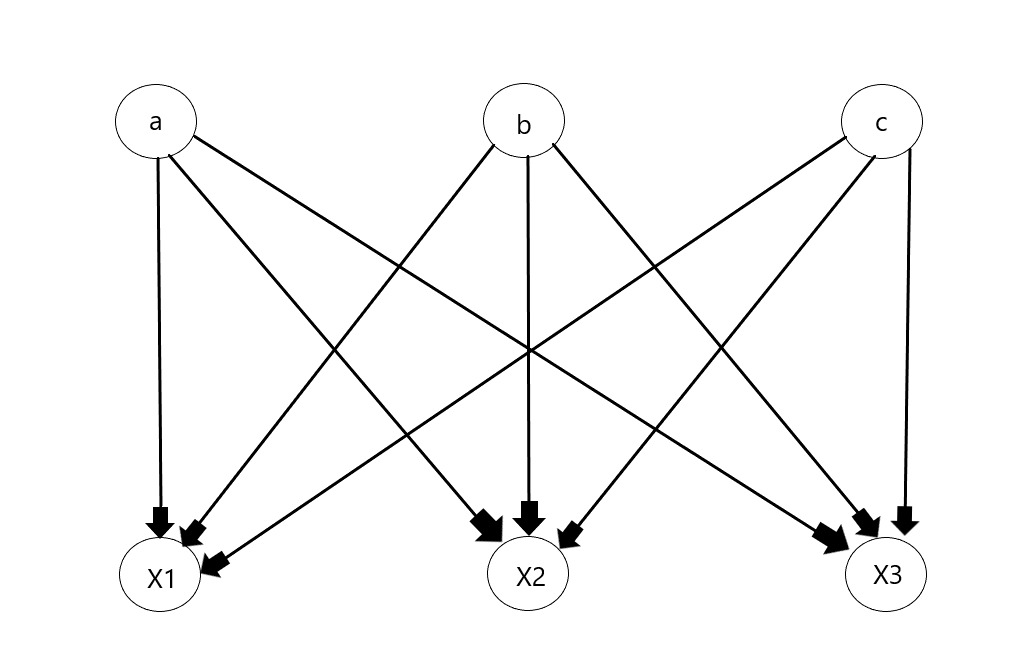
\includegraphics[width=0.5\linewidth]{q1_a.png}
                      \caption{The outcomes X1, X2 and X3 have an equal probability of landing either heads or tails}
                  \end{figure}

                  \begin{table}[H]
                      \caption{Bayesian network where a random variable C denoting which coin to draw has $X_1, X_2, X_3$ as child nodes.}
                      \begin{subtable}{.5\linewidth}
                          \centering
                          \begin{tabular}{|c|c|} \hline
                              \textbf{Coin} & \textbf{P(Coin)} \\ \hline
                              a             & 1/3              \\ \hline
                              b             & 1/3              \\ \hline
                              c             & 1/3              \\ \hline
                          \end{tabular}
                      \end{subtable}
                      \begin{subtable}{.5\linewidth}
                          \centering
                          \begin{tabular}{|c|c|c|} \hline
                              \textbf{Coin} & \textbf{$X_i$} & \textbf{P(Coin)} \\ \hline
                              a             & heads          & 0.2              \\ \hline
                              b             & heads          & 0.6              \\ \hline
                              c             & heads          & 0.8              \\ \hline
                          \end{tabular}
                      \end{subtable}
                  \end{table}
            \item
                  Given Information: $P(H) = \frac{2}{3}$ and $P(T) = \frac{1}{3}$. The probability for the three types of coins can
                  be calculated as $P(C|2\ heads, 1\ tails)$.

                  \begin{gather*}
                      P(C|2\ heads, 1\ tails) = P(2\ heads, 1\ tails|C)P(C) / P(2\ heads, 1\ tails) \\
                      \propto P(2\ heads, 1\ tails|C)P(C) \\
                      \propto P(2\ heads, 1\ tails)P(C) \\
                      P(X_1 = tails|C=a)P(X_2 =heads|C=a)P(X_3 = heads|C=a) \\= 0.8*0.2*0.2=0.032 \\
                      P(2\ heads, 1\ tails|C=a) = 3*0.032=0.096 \\
                      P(X_1 = tails|C=b)P(X_2 =heads|C=b)P(X_3 = heads|C=b) \\= 0.4*0.6*0.6=0.144 \\
                      P(2\ heads, 1\ tails|C=b) = 3*0.144=0.432 \\
                      P(X_1 = tails|C=c)P(X_2 =heads|C=c)P(X_3 = heads|C=c) \\= 0.2*0.8*0.8=0.128 \\
                      P(2\ heads, 1\ tails|C=c) = 3*0.128=0.384 \\
                  \end{gather*}

                  So, since $P(2\ heads, 1\ tails|C=b)$ has the highest probability among the three coins. So we can conclude coin b is
                  most likely to be drawn from the bag.
        \end{enumerate}
    \item[1.2]
        \begin{enumerate}
            \item
                  B = Burglary E = Earthquake
                  \begin{gather*}
                      P(B, E)=P(B|parents(B))P(E|parents(E))=P(B)P(E)
                  \end{gather*}

                  Therefore, Burglary and Earthquake are independent. \\ \\

                  A non-descendants shows that each variable is conditionally independent of each other.
                  The Bayesian network Burglary is a non-descendant of Earthquake therefore, is independent.

            \item
                  \begin{gather*}
                      P(B,E|A) = P(B|A) P(E|A) \\
                      P(A) = P(A|B,E)P(B)P(E) + P(A|B,\neg E)P(B)P(\neg E)  +  P(A|\neg B,E)P(\neg B)P(E) \\ + P(A| \neg B, \neg E)P(\neg B)P(\neg E) \\
                      =0.95*0.001*0.002+0.94*0.001*0.998+0.29*0.999*0.002+\\0.001*0.999*0.998 \\
                      P(A)=0.00251
                  \end{gather*}

                  \begin{gather*}
                      P(B|A) = P(A|B)P(B)/P(A) \\
                      =P(A|B,E)P(B)P(E) + P(A|B,\neg E)P(B)P(\neg E)/P(A) \\
                      =0.95*0.001*0.002+0.94*0.001*0.998/0.00251 \\
                      P(B|A)=0.37451
                  \end{gather*}

                  \begin{gather*}
                      P(E|A) = P(A|E)/P(A) \\
                      =P(A|E,B)P(B) + P(A|E,\neg B)P(\neg B)/P(A) \\
                      =P(A|B,E)P(B)P(E)+P(A|\neg B,E)P(\neg B)P(E)/P(A) \\
                      =0.95*0.001*0.002+0.29*0.999*0.002/0.00251 \\
                      P(E|A)=0.2316
                  \end{gather*}

                  \begin{gather*}
                      P(B|A)P(E|A)=0.37451*0.2316=0.0867 \\
                      P(B,E|A)=P(A|B,E)P(B,E)/P(A) \\
                      =P(A|B,E)P(B)P(E)/P(A) \\
                      =0.95*0.001*0.002/0.00251 \\
                      P(B,E|A)=0.000757
                  \end{gather*}

                  \begin{gather*}
                      P(B,E|A)=P(B|A)P(E|A) \\
                      0.000757 \neq 0.0867 \\
                  \end{gather*}

                  Therefore, if we observe Alarm = true, Burglary and Earthquake are not independent.
        \end{enumerate}
    \item[1.3]
        \begin{enumerate}
            \item
            \item
        \end{enumerate}
    \item[1.4]
        \begin{enumerate}
            \item Determine if the following are to be asserted by the network structure.
                  \begin{enumerate}
                      \item \[P(B,I,M)=P(B)P(I)P(M)\] Is not asserted because you would I, B, M would need to have independent paths with each other.
                      \item \[P(J|G) = P(J|G,I)\] Is asserted
                      \item \[P(M|G,B,I) = P(M|G,B,I,J)\] Is asserted
                  \end{enumerate}
            \item
                  \begin{gather*}
                      P(b,i,\neg m, g, \neg j) = P(b)P(\neg m) P(i|b, \neg m) P(g|b,i, \neg m) P(\neg j|g) \\
                      = 0.9*0.9*0.5*0.8*0.1 = 0.0324
                  \end{gather*}
            \item
                  \begin{gather*}
                      P(j|b,\neg i,m)=P(g|b, \neg i, m)P(j|g)+P(\neg g|b, \neg i, m)P(j|\neg g)/ \\
                      P(g|b, \neg i, m)P(j|g) + P(\neg g|b, \neg i,m)P(j|\neg g) + P(g|b, \neg i, m) \\
                      P(\neg j|g)+P(\neg g|b, \neg i, m)P(\neg j|\neg g)\\
                      P(j|b, \neg i, m) = 0.0*0.9+1*0.0/0.0*0.9+1*0.0+1+1*1 = 0
                  \end{gather*}
        \end{enumerate}
    \item[1.5]
        \begin{enumerate}
            \item
            \item
                  \begin{gather*}
                      P(E_0) = <0.7, 0.3> \\
                      P(E_1) = \sum\limits_{E_0}P(E_1|E_0)P(E_0) \\
                      = (<0.8,0.2>0.7 + <0.3,0.7>0.3) \\
                      = <0.65, 0.35> \\
                      P(E_1|e_1)=P(e_1|E_1)P(E_1) \\
                      = <0.8*0.9,0.3*0.7><0.65,0.35> \\
                      = <0.72, 0.21><0.65,0.35> \\
                      = <0.468, 0.0735> \\
                      0.468+0.0735 = 0.5415 \\
                      =<0.468/0.5415, 0.0735/0.5415> \\
                      =<0.8643, 0.1357> \\
                      P(E_2|e_1) = \sum\limits_{E_1}P(E_2|E_1)P(E_1|e_1) \\
                      =<0.7321, 0.2679> \\
                      P(E_2|e_{1:2})=P(e_2|E_2)P(E_2|e_1) \\
                      = <0.5010, 0.4990> \\
                      P(E_3|e_{1:2})=\sum\limits_{E_3}P(E_3|E_2)P(E_2|e_{1:2}) \\
                      = <0.5505,0.4495> \\
                      P(E_3|e_{1:3})=P(e_3|E_3)P(E_3|e_{1:2}) \\
                      = <0.1045, 0.8955>
                  \end{gather*}
        \end{enumerate}
\end{enumerate}


\end{document}